
\chapter{Opis projektnog zadatka}
		
		\textbf{\textit{dio 1. revizije}}\\
		
		
		Cilj ovog projekta je izgradnja web aplikacije koja će omogućiti ljudima/bolesnicima lakše prijavljivanje na slobodne termine za medicinsku rehabilitaciju i fizikalnu terapiju te praćenje njihovog zdravstvenog napretka. Također će omogućiti zaposlenicima ustanove da odbijaju ili prihvaćaju termine ovisno o raspoloživosti prostorija, opreme i osoblja pritom imajući mogućnost uvida u pacijentove prošle terapije i napredak. Vrijeme porovođenja rehabilitacije je svakim radnim danom od ponedjeljka do petka od 8:00 do 20:00 sati.
		
		\noindent Aplikacija će razlikovati tri vrste korisnika: 
		\begin{packed_item}
			
			\item  pacijenta/bolesnika
			\item  liječnika - djelatnika zdravstvene ustanove
			\item  administratora
		\end{packed_item}
		
		Prilikom pokretanja web aplikacije svaki korisnik unosi svoj e-mail i lozinku. Ovisno o vrsti korisnika biti će preusmjereni na različite stranice.
		
		\textit{Pacijent} se samostalno prijavljuje u sustav. U slučaju da još ne postoji imati će opciju registracije. Za registraciju mora unijeti: 
		\begin{packed_item}
			\item ime
			\item prezime
			\item e-mail adresu
			\item MBO - Matični Broj Osiguranika
			\item broj telefona
			\item lozinku
		\end{packed_item}
		Prilikom registracije pomoću MBO-a provjerava se ako korisnik postoji u središnjem informacijskom sustavu zdravstvene zaštite.
		Nakon prijave ili registracije korisnik je preusmjeren na stranicu gdje se prikazuju njegovi termini i zahtjevi. U terminima se prikazuju protekli i budući termini, za protekle termine piše ako je pacijent došao te komentari djelatnika ustanove o napretku. Termin se dobiva nakon što se odobri zahtjev za jednim.		
		Zahtjev se sastoji od:
		\begin{packed_item}
			\item vremena predaje
			\item željenog termina
			\item vrste/tipa rehabilitacije
			\item liječnika koji je uputio pacijenta na terapiju
			\item reference na prošlu terapiju
			\item statusa
		\end{packed_item}
		Status može biti odobreno, odbijeno, čeka na odobrenje ili isteklo u slučaju da nitko nije odobrio niti odbio termin do željenog vremena terapije.
		Klikom na opciju \textit{naruči se} pacijent može napraviti novi zahtjev za terminom. Zahtjev popunjava unoseći vrstu rehabilitacije, liječnika koji ga je uputio, ukoliko se radi o ponovljenoj terapiji odabrati će i termin već obavljenog postupka terapije u ustanovi, također u komentar za liječnika dodaje opis svojih oboljenja. Status liječnika koji je izdao uputnicu provjerava se u imeniku liječnika. U odabiru termina biti će prikazano prvih nekoliko slobodnih termina za odabrani tip rehabilitacije i opcije da se unese željeni datum i vrijeme. Nakon odabira željenog termina pacijent predaje zahtjev. Pacijent će o odobrenju ili odbijanju zahtjeva, kao i svim mogućim promjenama biti obaviješten mailom.
		
		\textit{Liječnik} nakon prijavljivanja u sustav ima pregled svih pacijenata i njihovih podataka, klikom na prikaz terapije bit će mu prikazani svi termini odabranog pacijenta i detalji o njima, tu će imati opciju evidentirati dolazak pacijenta i zabilježiti komentare vezane uz napredak ili pregledati napredak i komentare iz prošlih termina. Također svaki djelatnik ustanove imati će mogućnost prihvaćanja ili odbijanja termina ovisno o raspoloživosti prostorija i opreme. Liječnik koji prihvati zahtjev automatski će se dodati kao liječnik koji će tu terapiju izvoditi. 
		
		\textit{Administrator} ima pregled svih pacijenata i djelatnika. Uz ovlasti koje imaju djelatnici administrator pri zaposlenju novog liječnika izrađuje korisnički račun za njega s inicijalnom lozinkom. Također nakon prestanka radnog odnosa administrator može ukloniti tog liječnika. Administrator definira sve što je potrebno za ispravan rad sustava, dakle može mijenjati broj opreme, dostupne prostorije.
		
		Ovim projektom smanjio bi se opseg posla djelatnika ustanove 
		---
		
		Aplikacija će se moći proširiti da djelatnici uopće ne moraju prihvaćati ili odbijati prijave, već će to sustav raditi automatski na temelju raspoloživih podataka o opremi, prostorijama, djelatnicima i već zauzetim terminima. Svi termini, prostorije, oprema i djelatnici vidljivi su adminu koji im može mijenjati status za određeno vrijeme, na primjer kada liječnik ode na godišnji odmor može promijeniti njegov status u neaktivan za to razdoblje ili kada cijela ustanova ima sastanak onemogućiti sve termine za vrijeme tog sastanka. Ostala bi mogućnost upućivanja maila ili telefonskog poziva pacijentu u slučaju ikakvih promjena. 
		
		
		---
		
	
		
		\begin{packed_item}
			\item \textit{potencijalna korist ovog projekta}
			\item \textit{postojeća slična rješenja (istražiti i ukratko opisati razlike u odnosu na zadani zadatak). Dodajte slike koja predočavaju slična rješenja.}
			\item \textit{skup korisnika koji bi mogao biti zainteresiran za ostvareno rješenje.}
			\item \textit{mogućnost prilagodbe rješenja }
			\item \textit{opseg projektnog zadatka}
			\item \textit{moguće nadogradnje projektnog zadatka}
		\end{packed_item}
		
		\textit{Za pomoć pogledati reference navedene u poglavlju „Popis literature“, a po potrebi konzultirati sadržaj na internetu koji nudi dobre smjernice u tom pogledu.}
		\eject
		
		\section{Primjeri u \LaTeX u}
		
		\textit{Ovo potpoglavlje izbrisati.}\\

		U nastavku se nalaze različiti primjeri kako koristiti osnovne funkcionalnosti \LaTeX a koje su potrebne za izradu dokumentacije. Za dodatnu pomoć obratiti se asistentu na projektu ili potražiti upute na sljedećim web sjedištima:
		\begin{itemize}
			\item Upute za izradu diplomskog rada u \LaTeX u - \url{https://www.fer.unizg.hr/_download/repository/LaTeX-upute.pdf}
			\item \LaTeX\ projekt - \url{https://www.latex-project.org/help/}
			\item StackExchange za Tex - \url{https://tex.stackexchange.com/}\\
		
		\end{itemize} 	


		
		\noindent \underbar{podcrtani tekst}, \textbf{podebljani tekst}, 	\textit{nagnuti tekst}\\
		\noindent \normalsize primjer \large primjer \Large primjer \LARGE {primjer} \huge {primjer} \Huge primjer \normalsize
				
		\begin{packed_item}
			
			\item  primjer
			\item  primjer
			\item  primjer
			\item[] \begin{packed_enum}
				\item primjer
				\item[] \begin{packed_enum}
					\item[1.a] primjer
					\item[b] primjer
				\end{packed_enum}
				\item primjer
			\end{packed_enum}
			
		\end{packed_item}
		
		\noindent primjer url-a: \url{https://www.fer.unizg.hr/predmet/proinz/projekt}
		
		\noindent posebni znakovi: \# \$ \% \& \{ \} \_ 
		$|$ $<$ $>$ 
		\^{} 
		\~{} 
		$\backslash$ 
		
		
		\begin{longtblr}[
			label=none,
			entry=none
			]{
				width = \textwidth,
				colspec={|X[8,l]|X[8, l]|X[16, l]|}, 
				rowhead = 1,
			} %definicija širine tablice, širine stupaca, poravnanje i broja redaka naslova tablice
			\hline \SetCell[c=3]{c}{\textbf{naslov unutar tablice}}	 \\ \hline[3pt]
			\SetCell{LightGreen}IDKorisnik & INT	&  	Lorem ipsum dolor sit amet, consectetur adipiscing elit, sed do eiusmod  	\\ \hline
			korisnickoIme	& VARCHAR &   	\\ \hline 
			email & VARCHAR &   \\ \hline 
			ime & VARCHAR	&  		\\ \hline 
			\SetCell{LightBlue} primjer	& VARCHAR &   	\\ \hline 
		\end{longtblr}
		

		\begin{longtblr}[
				caption = {Naslov s referencom izvan tablice},
				entry = {Short Caption},
			]{
				width = \textwidth, 
				colspec = {|X[8,l]|X[8,l]|X[16,l]|}, 
				rowhead = 1,
			}
			\hline
			\SetCell{LightGreen}IDKorisnik & INT	&  	Lorem ipsum dolor sit amet, consectetur adipiscing elit, sed do eiusmod  	\\ \hline
			korisnickoIme	& VARCHAR &   	\\ \hline 
			email & VARCHAR &   \\ \hline 
			ime & VARCHAR	&  		\\ \hline 
			\SetCell{LightBlue} primjer	& VARCHAR &   	\\ \hline 
		\end{longtblr}
	


		
		
		%unos slike
		\begin{figure}[H]
			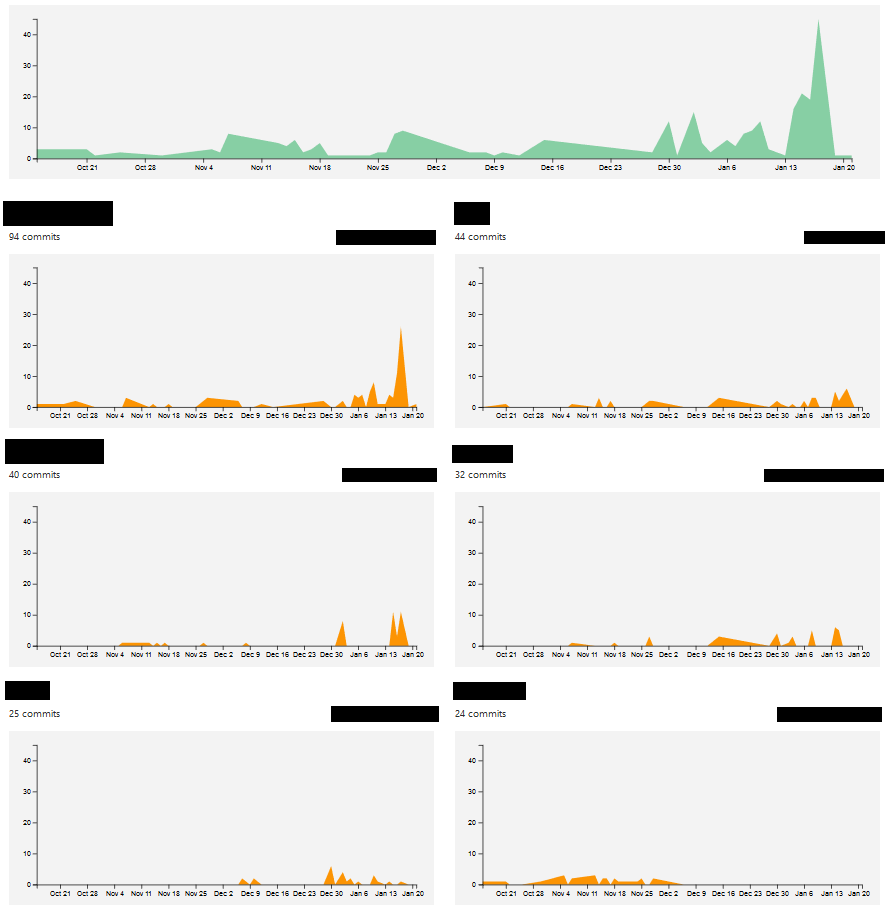
\includegraphics[scale=0.4]{slike/aktivnost.PNG} %veličina slike u odnosu na originalnu datoteku i pozicija slike
			\centering
			\caption{Primjer slike s potpisom}
			\label{fig:promjene}
		\end{figure}
		
		\begin{figure}[H]
			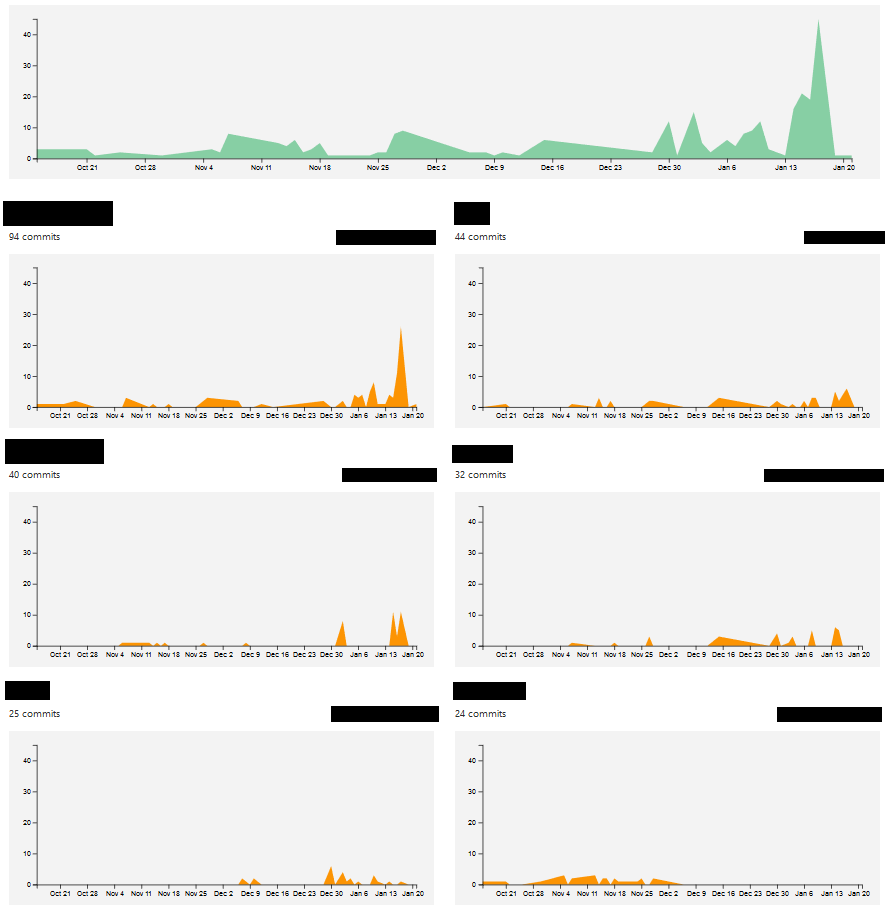
\includegraphics[width=\textwidth]{slike/aktivnost.PNG} %veličina u odnosu na širinu linije
			\caption{Primjer slike s potpisom 2}
			\label{fig:promjene2} %label mora biti drugaciji za svaku sliku
		\end{figure}
		
		Referenciranje slike \ref{fig:promjene2} u tekstu.
		
		\eject
		
	